\subsection{Evaluating Performance Comparison Results}


COHEN:
\textbf{How did the program performance compare to its selected standard?} 
\textbf{Did the program demonstrate good performance?}
\textbf{Is the programs performance different from predictions?} 
\textbf{Did you learn what you wanted from the programs experiments?}

The best route set, having four routes, constructed by the proposed algorithm using parameter values presented in presented in Table \vref{table:performanceComparison_bestRouteSet4} and Fig. \vref{fig:bestRouteSet4}.  The best route set, having four routes, constructed by the plain ACO implementation is found in Table \vref{table:performanceComparison_bestRouteSet4_ACO}. Table \vref{table:performanceComparison_ACOSSOBEST} compares the average produced results of these two algorithms, and the best, worst, average, median and STD results is presented in Appendix \ref{appendixC}, Table \vref{table:performanceComparison_ACOFull}.

When it comes to comparing the proposed algorithm with the plain ACO implementation, As seen in Table \vref{table:performanceComparison_ACOSSOBEST}, the SSO produce better results than the plain ACO implementation. We did expect SSO to be better. ACO has, as mentioned, a known limitation of getting stuck at a local optima. This is very well demonstrated in Figure \ref{fig:acovssso}, which shows the average growth in the $TOTFIT$ value for each iteration of ACO and SSO. (10 runs for each algorithm is run. For each iteration, the average $TOTFIT$ value among each run is recorded.) As one can observe, the ACO implementation manage to find good solutions fast, by following pheromone trails laid by previous ants. But after around 35 iterations, the algorithm is unable to find better solutions. The amount of pheromone on the first best paths only increase, and unable ants to explore possible better routes. 

As one can see, the proposed SSO algorithm manage to get out of this inconvenience. One reason to this is that in the plain ACO implementation: the ants do not have memory. The memory function will make more route sets based on the constraints, because it remembers where it has been before. The removal makes ACO produce less route sets - where it could have produced more good route sets. As seen in the parameter settings experiments, the reason SSO is better is also because of the CA and AF parameters. Rewarding the best route sets, by making followers walk the same paths as the best route sets, and with this giving these paths more pheromone by the pb parameter. As seen in the parameter settings experiments, the algorithm do produce better results with these additional parameters. The notion of best global solution can also a reason, the edges walked by the best ants will give the edge a higher probability of being selected. To unable the ants at getting stuck at a local optima Crazy ants explore new route sets and can with this explore possible better solutions than paths walked in early iterations which has gained a lot of pheromone. This additional features can bee a reason that SSO is better. 
% Notion of global best solution, crazy ants, following ants reward best edges, memory etc.

 \begin{figure}[H]
    \begin{center}
    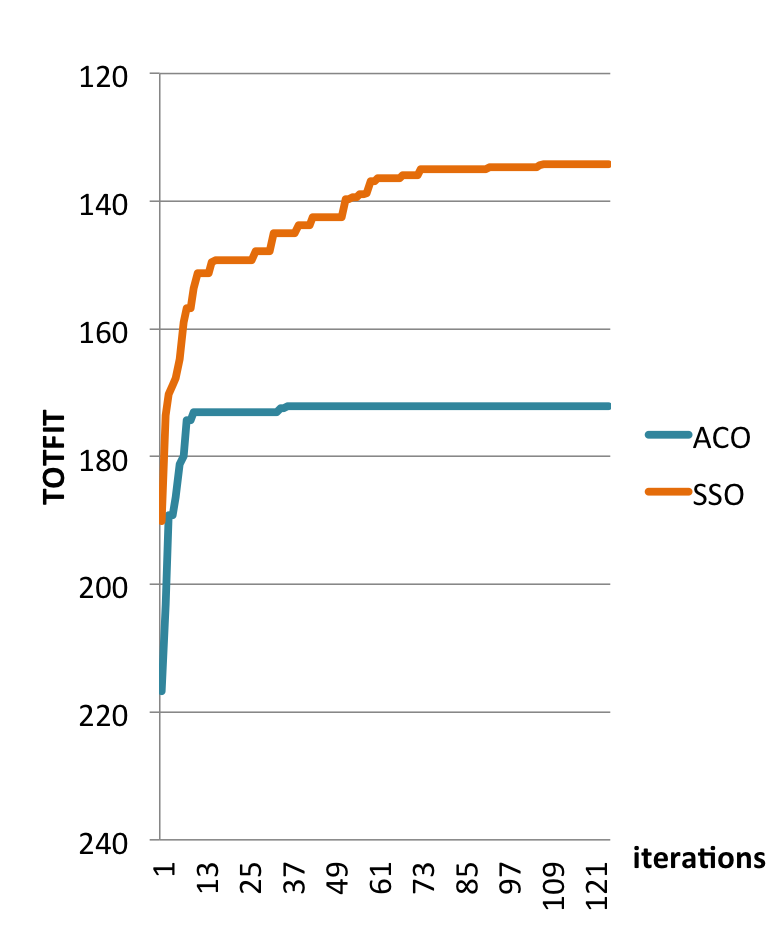
\includegraphics[width=3in]{assets/acovsssoNEW.png}
    \end{center}
    \caption{Evolution of TOTFIT for ACO and SSO }
    \label{fig:acovssso} 
\end{figure}

In Table \vref{table:performanceComparison_4}, the results of the SSO, having four routes, are compared with the respective experimental results published in the literature. As presented in Table \vref{table:performanceComparison_4}, the route set constructed by SSO has lower ATT compared to all route sets constructed by other approaches. The values of the rest of the performance criteria $d_0, d_1, d_2, d_{unstat}$, route sets constructed by almost all, except \citep{mandl79, kidwai98, chakroborty02}, produce better results concerning number direct travelers. 

The low value of ATT is due to the weighting parameter of f.. The other approaches has sat this to favor d0 - leses mer om dette. This is due to the user set parameters is .. and ATT is favored against traveling directly. In the other \emph{\color{blue} TODO} the weights for parameters F1, F2 and F3, which together is the TOTFIT value, is weighted the same. The best produced TOTFIT, does not mean it only selects route sets with the lowest ATT, it will still select the once with one of the best produced d0. But the ratio against these two parameters favourise a low ATT against a low d0. The weight parameter, $\sigma$, explained in \vref{sec:f1}, is a user defined parameter used to control the importance of $Fi$. In this solution this is sat to favor $ATT$. This is demonstrated in Fig. [som skal lages], When traveling from node7 to node14 the passenger would have to change route from route 4 to route 3 at node 10 and the traveling time will be 20 mins including transfer penalties. If the algorithm would favour route 1, which travels dirctly from node 7 to node 14, the traveling time would be 27 minutes - increasing the ATT.

The best route set, having six routes, constructed by the proposed algorithm is presented in Table \vref{table:performanceComparison_bestRouteSet6} and Fig. \vref{fig:bestRouteSet6}. 
Evaluate.

The best route set, having seven routes, constructed by the proposed algorithm is presented in Table \vref{table:performanceComparison_bestRouteSet7} and Fig. \vref{fig:bestRouteSet7}. 
Evaluate

The best route set, having eight routes, constructed by the proposed algorithm is presented in Table \vref{table:performanceComparison_bestRouteSet8} and Fig. \vref{fig:bestRouteSet8}.
Evaluate

As one can observe in \vref{table:performanceComparison_routesets}, the amount of direct travelers increase with in line with the number of route sets. This makes sense because thus more route sets the passenger can choose from, thus bigger probability for the passenger to find a route that is convenient for him / her. This is well demonstrated when comparing the graphs of four route sets, \vref{fig:bestRouteSet4}, and six route sets, Figure \vref{fig:bestRouteSet6}, and seven route sets. However, as one can see in route sets eight. It has reached a threshold \emph{\color{blue} TODO: må vente på resultater fra sso8}.

 \begin{table}[H]
    \centering
    \begin{tabular}{|l||l|l|l|l|l|}
    \hline
    Route Set & $d_0(\%)$ & $d_1(\%)$ & $d_2(\%)$ & $d_{unsat}(\%)$ & $ATT$ \\
    \hline
    4 & 85.21 & 13.49 & 1.30 & 0.00 & 10.27\\
    6 & 87.17 & 12.0 & 0.82 & 0.01 & 10.11\\
    7 & 88.49 & 10.72 & 0.79 & 0.0 & 10.08\\
    8\\
    \hline
    \end{tabular}
    \caption {Evaluating increase of Route Sets}
    % 50 runs
    \label{table:performanceComparison_routesets}
\end{table}

